%
% Einfache LaTeX-Vorlage f�r Arbeiten am Lehrstuhl Kranzlm�ller / MNM-Team
% - optimiert f�r die Arbeit mit g�ngigen LaTeX-Editoren
% - funktioniert ohne Makefile und Anpassungen der LaTeX-Verzeichnisstruktur
% - verwendet Komaskript f�r ein (nach europ�ischen Gepflogenheiten) sch�neres Layout
% 
% v1, 2007 (Michael Brenner)
% Diese Version: v1.1, 2012 (Michael Brenner)
% Diese Version: v1.2, 2017 (Michael Brenner)
% 


\documentclass[bibliography=totoc,listof=totoc,BCOR=5mm,DIV=12]{scrbook} % Rand f�r Bindung: 5mm / falls Index verwendet, erg�nze "index=totoc" zu den Optionen 
\usepackage[latin1]{inputenc} % Umlaute im Text
\usepackage{graphicx} % Einf�gen von Grafiken  - f�r PDF-Latex: .pdf und .png (.jpg m�glich, sollte aber vermieden werden)
\usepackage{url}           % URL's (z.B. in Literatur) sch�ner formatieren
\usepackage{hyperref} % sorgt f�r f�r Hyperlinks in PDF-Dokumenten
\usepackage{color}
\usepackage{listings}
\usepackage{color}

\definecolor{lightgray}{rgb}{0.5,0.5,0.5}
\definecolor{gray}{rgb}{0.5,0.5,0.5}
\definecolor{mauve}{rgb}{0.58,0,0.82}

\lstset{frame=tb,
  language=C++,
  aboveskip=6mm,
  belowskip=6mm,
  showstringspaces=false,
  columns=flexible,
  basicstyle={\small\ttfamily},
  numbers=left,
  numbersep=5pt,
  numberstyle=\tiny\color{gray},
  keywordstyle=\color{blue},
  commentstyle=\color{lightgray},
  stringstyle=\color{mauve},
  breaklines=true,
  breakatwhitespace=true,
  tabsize=3
}

\newtheorem{defi}{Definition}[chapter]

\graphicspath{{./Bilder/}}

%
% der Befehl \hypenation versteht keine Sonderzeichen, also weder �
% noch "a noch \"a. W�rter die derartige Zeichen enthalten m�ssen
% direkt im Text getrennt werden, z.B. W�r\-ter
%
\hyphenation{Ma-nage-ment}
\hyphenation{Ma-nage-ment-agent}
\hyphenation{Ma-nage-ment-agent-en}
\hyphenation{Ma-nage-ment-ar-chi-tek-tur}
\hyphenation{Ma-nage-ment-ar-chi-tek-tu-ren}
\hyphenation{Ma-nage-ment-an-wen-dung}
\hyphenation{Ma-nage-ment-an-wen-dung-en}
\hyphenation{Ma-nage-ment-an-for-der-ung}
\hyphenation{Ma-nage-ment-funk-ti-on}
\hyphenation{Ma-nage-ment-funk-ti-onen}
\hyphenation{Ma-nage-ment-kon-zep-te}
\hyphenation{Ma-nage-ment-res-source}
\hyphenation{Ma-nage-ment-in-for-ma-ti-on}
\hyphenation{Ma-nage-ment-res-sour-cen}
\hyphenation{ma-nage-ment-re-le-vante}
\hyphenation{ma-nage-ment-sy-stem}
\hyphenation{ma-nage-ment-sy-steme}
\hyphenation{Ma-nage-ment-in-stru-men-tie-rung}
\hyphenation{Ma-nage-ment-platt-form}
\hyphenation{Sys-te-men}
\hyphenation{Sys-tem-um-ge-bun-gen}
\hyphenation{Sys-tem-ma-nage-ment}
\hyphenation{DHCP}
\hyphenation{Ma-nage-ment-diszi-plinen}
\hyphenation{System-management-architekturen}
\hyphenation{Verwendungs-nachweise}
\hyphenation{Video-einricht-ungen}
\hyphenation{Res-source}
\hyphenation{Res-sourcen}
\hyphenation{Grund-anwendung}
\hyphenation{Grund-anwendungen}
\hyphenation{Basis-anwendung}
\hyphenation{Core}
\hyphenation{Kom-mu-ni-ka-ti-on}
\hyphenation{De-sign-ent-schei-dung}
\hyphenation{Sprung-ad-res-sen}
\hyphenation{Klas-si-fi-ka-ti-on}
\hyphenation{Schreib-recht}
\hyphenation{Be-nut-zer-zer-ti-fi-kat}
\hyphenation{Bau-stein-ent-wi-ckler}
\hyphenation{ad-mi-ni-stra-ti-ve}

 % in dieses File kommen W�rter die Latex nicht richtig trennt

\begin{document}

% ---------------------------------------------------------------
\frontmatter % Titelbl�tter und Erkl�rung jeweils spezifisch f�r die jeweilige Uni einbinden
    %%%%%%%%%%%%%%%%%%%%%%%%%%%%%%%
% erste Seite

\thispagestyle{empty}

\begin{center}

\vspace*{-2cm}

{\Huge INSTITUT F�R INFORMATIK\\[1mm]}
DER LUDWIG--MAXIMILIANS--UNIVERSIT�T M�NCHEN\\

\vspace*{1cm}


\includegraphics[width=0.3\textwidth]{lmu_siegel}

\vspace*{2cm}

{\Large \textbf{Master's Thesis}}\\ % oder Fortgeschrittenenpraktikum, Master's Thesis, Bachelorarbeit etc.

\vspace{2.0cm}
{\Huge \textbf{C++ Graph Concepts for}}\\
\vspace*{3mm}
{\Huge \textbf{Partitioned Global Address Space}}\\
\vspace*{20mm}

{\LARGE Stefan Effenberger} % Name des Autors

\vspace{3cm}
\end{center}

\newpage

%%%%%%%%%%%%%%%%%%%%%%%%%%%%%%%
% zweite Seite

\thispagestyle{empty}
\cleardoublepage

%%%%%%%%%%%%%%%%%%%%%%%%%%%%%%%
% dritte Seite (Kopie der ersten)

\thispagestyle{empty}

\begin{center}

\vspace*{-2cm}

{\Huge INSTITUT F�R INFORMATIK\\[1mm]}
DER LUDWIG--MAXIMILIANS--UNIVERSIT�T M�NCHEN\\

\vspace*{1cm}


\includegraphics[width=0.3\textwidth]{lmu_siegel}

\vspace*{2cm}

{\Large \textbf{Master's Thesis}}\\ % oder Fortgeschrittenenpraktikum, SEP etc.

\vspace{2.0cm}
{\Huge \textbf{C++ Graph Concepts for}}\\
\vspace*{3mm}
{\Huge \textbf{Partitioned Global Address Space}}\\
\vspace*{20mm}

{\LARGE Stefan Effenberger} % Name des Autors
\vspace{2cm}

\parbox{1cm}{
\begin{large}
\begin{tabbing}
Aufgabensteller: \hspace{.5cm} \=Prof. Dr. Dieter Kranzlm�ller\\[2mm]
Betreuer:
\>Tobias Fuchs\\[5mm]
Abgabetermin: \> \textcolor{red}{ADD DATE}\\
\end{tabbing}
\end{large}}\\
\vspace{5mm}

\end{center}
 % Titelbl�tter LMU - auskommentieren falls TUM-Arbeit
%    % Richtlinien, siehe http://wwwpa.in.tum.de/generell/Abschlussarbeitsform.html
%
%%%%%%%%%%%%%%%%%%%%%%%%%%%%%%%


% Deckblatt

\thispagestyle{empty}

\begin{center}
    
\includegraphics[width=3cm]{tum-logo}\\
    \vspace{.5cm}
% "Technische Universit�t M�nchen" oder alternativ das Logo der TUM
    {\Large \sc Technische Universit�t M�nchen}\\

    \vspace{1cm}
% "Fakult�t f�r Informatik"
    {\Huge \sc Fakult�t f�r Informatik\\[1mm]}


    \vspace{2cm}
% Diplomarbeit | Master's Thesis | Bachelorarbeit in Informatik | Wirtschaftsinformatik |
    {\Large \textbf{Masterarbeit in Informatik}}\\
% Thema bzw. Titel der Arbeit  (In der Sprache, in der die Arbeit verfasst wurde)
    \vspace{2.0cm}
    {\Huge \textbf{Ein Lorem-Rahmenwerk}}\\ % bei langen Titeln ggf. Schriftgr��e auf \huge herunter setzen
    \vspace*{3mm}
    {\Huge \textbf{f�r Ipsum-Systeme}}\\
    \vspace*{3mm}
    {\Huge \textbf{-- ein Dolor-Ansatz}}\\
    \vspace{1.5cm}
% Vorname und Nachname des Bearbeiters/ der Bearbeiterin
    Vorname Nachname

    \vspace{5cm} % ggf. je nach Zeilenzahl und Schriftgr��e des Titels anpassen
    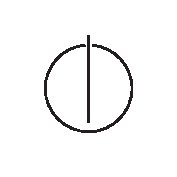
\includegraphics[width=2.4cm]{tum-info-logo}
\end{center}

\newpage

%%%%%%%%%%%%%%%%%%%%%%%%%%%%%%%
% R�ckseite Deckblatt

\thispagestyle{empty}
\cleardoublepage

%%%%%%%%%%%%%%%%%%%%%%%%%%%%%%%
% Erste Seite (Titelblatt)

\thispagestyle{empty}

\begin{center}

    
\includegraphics[width=3cm]{tum-logo}\\
    \vspace{.5cm}
    {\Large \sc Technische Universit�t M�nchen}\\


    \vspace{.5cm}

    {\huge \sc Fakult�t f�r Informatik\\[1mm]}


    \vspace{1cm}

    {\Large \textbf{Diplomarbeit in Informatik}}\\ % oder SEP etc.

% Thema bzw. Titel der Arbeit  (In der Sprache, in der die Arbeit verfasst wurde)
    \vspace{1.5cm}
    {\huge \textbf{Ein Lorem-Rahmenwerk}}\\ % bei langen Titeln ggf. Schriftgr��e herunter setzen
    \vspace*{3mm}
    {\huge \textbf{f�r Ipsum-Systeme}}\\
    \vspace*{3mm}
    {\huge \textbf{-- ein Dolor-Ansatz}}\\

% die englische bzw. deutsche Entsprechung des Titels
    \vspace{1cm}
    {\huge \textbf{A Lorem Framework}}\\ % bei langen Titeln ggf. Schriftgr��e herunter setzen
    \vspace*{3mm}
    {\huge \textbf{for Ipsum Systems}}\\
    \vspace*{3mm}
    {\huge \textbf{-- a Dolor Approach}}\\
    \vspace{1cm}

    \parbox{1cm}{
      \begin{large}
        \begin{tabbing}
          Bearbeiter: \hspace{1.5cm}
            \=Vorname Nachname\\[2mm]
    Aufgabensteller: \>Prof. Dr. Dieter Kranzlm�ller\\[2mm]
    Betreuer: \>MNM-Team-Betreuer 1\\ % alphabetische Reihenfolge (Nachname)
    \>MNM-Team-Betreuer 2\\
    \>Externer Betreuer 1 (Firma)\\[5mm]
    Abgabedatum: \> 7. Juli 2077\\
        \end{tabbing}
      \end{large}
    }\\

    \vspace{.3cm}

    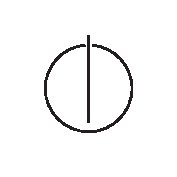
\includegraphics[width=2.4cm]{tum-info-logo}

\end{center}
 % Titelbl�tter TUM - auskommentiert lassen falls LMU-Arbeit
    \thispagestyle{empty}
    \cleardoublepage
    %
% LaTeX-Rahmen f�r Arbeiten am Lehrstuhl Hegering
%
% Harald Roelle, 2001, 2002
%
% basierend auf Arbeiten von Helmut Reiser, Boris Gruschke und Stephen Heilbronner
%

\newpage

\thispagestyle{empty}

\begin{large}

\vspace*{2cm}

\noindent
Hiermit versichere ich, dass ich die vorliegende Masterarbeit
selbst�ndig verfasst und keine anderen als die angegebenen Quellen
und Hilfsmittel verwendet habe.

\vspace{2cm}

\noindent
M�nchen, den \textcolor{red}{ADD DATE}

\vspace{3cm}

\hspace*{7cm}%
\dotfill\\
\hspace*{8.5cm}%
\textit{(Unterschrift des Kandidaten)}

\end{large}
 % Erkl�rung (Arbeit selbstst�ndig verfasst) - auskommentieren falls TUM-Arbeit
%    \begin{large}

\vspace*{2cm}
\noindent
Ich versichere, dass ich diese Masterarbeit % (bzw. Master's Thesis)
selbst�ndig verfasst und nur die angegebenen Quellen und Hilfsmittel verwendet habe.

\vspace{2cm}

\noindent
M�nchen, den 7. Juli 2077

\vspace{3cm}

\hspace*{7cm}%
\dotfill\\
\hspace*{8.5cm}%
\textit{(Unterschrift des Kandidaten)}

\end{large}
 % Erkl�rung (Arbeit selbstst�ndig verfasst) - auskommentiert lassen falls LMU-Arbeit
    \thispagestyle{empty}
    \cleardoublepage
    \vspace*{2cm}

\begin{center}
    \textbf{Abstract}
\end{center}

\vspace*{1cm}

\noindent Hier steht eine kurze Zusammenfassung der Arbeit. Sie darf auf gar keinen Fall
l�nger als eine Seite sein, ca. eine drittel bis eine halbe Seite ist optimal.

 % Abstract
    \thispagestyle{empty}
    \tableofcontents % Inhaltsverzeichnis

% ---------------------------------------------------------------
\mainmatter % die eigentliche Arbeit

\chapter{Introduction}
Many scientific projects are largely enabled by simulation. Because such simulations often require huge computational capabilites, single compute nodes with a shared-memory architecture cannot provide enough computation power and storage for numerous cases. For this reason, in High Performance Computing (HPC), work is distributed among multiple, interconnected nodes to facilitate the solving of large problems in a timely manner. Since processors cannot directly access the memory of other nodes, the traditional programming model for such systems requires programmers to explicitly distribute data between nodes via message passing. This imposes high demands on the programming skills of scientists who might not have a background in computer science.

Therefore, with the Partitioned Global Address Space (PGAS) model, a new approach is proposed: The memory space of individual nodes in a system is unified within a global address space so that each node can directly access the memory of all other nodes. Programmers are still required to keep data access between nodes to a minimum because data transferal over an interconnect is costly. To further reduce the demands on the programmer, distributed data structures that handle data distribution and load balancing are needed.

Furthermore, data-intensive tasks have been gaining a continually growing interest in the scientific community. Traditionally, applications in HPC follow a computation-centric approach by solving numerical algorithms in the fastest possible way. As ``Big Data'' is becoming increasingly important in scientific projects, a shift towards more data-oriented applications can be observed in recent HPC projects \cite{fusionfs}. This trend requires distributed data structures that allow for the storage of large amounts of irregular data and cater to the needs of ever-changing dynamic data.

\section{Problem statement}
Data can be represented in numerous ways. The most generic form of data representation is enabled by \textit{graphs}. A graph G(V, E) is a pair with a set of vertices V and a set of edges E that connect the vertices. This allows for the representation of data and its relationships in regular as well as irregular patterns.

On distributed machines, graph data structures can be implemented using a variety of different characteristics. This has lead to many different implementations - usually a new implementation for each algorithm - which are hardly compatible with each other. To overcome this situation, generic programming abstractions to facilitate reuse of existing code and to lower the demands on programmers are needed.

As of today, no generic graph abstractions implementing the PGAS model exist. This work therefore aims to provide a graph abstraction for C++ containers that allows for the implementation of arbitrary graph algorithms following the PGAS model on distributed memory machines.

\section{Scope and Objectives}
In this work, a C++ concept for graph containers following the PGAS model is presented. The concept is part of the DASH C++ Template Library and thus uses concepts already present in the library. 

The graph concept is meant to provide a generic framework for the programming of arbitrary graph algorithms in the context of distributed machines and especially the Partitioned Global Address Space model. This means that it meets the following requirements:

\begin{itemize}  
\item Native support for one-sided communication
\item Support for the programming of synchronous graph algorithms
\item Support for the programming of asynchronous graph algorithms
\item Portability across platforms (\textcolor{red}{PORTABLE EFFICIENCY?})
\item Support for heterogenous systems
\item \textcolor{red}{FINISH REQUIREMENTS}
\end{itemize}

Furthermore, this work provides concepts for the dynamic allocation of graph data across multiple machines with a focus on optimized data locality. \textcolor{red}{LOAD BALANCING?}

A reference implementation is then used to verify the usability, correctness and universality of the given concepts. While the concepts are designed for high performance, the reference implementation is not. This means that the evaluation of this implementation does not account for the performance of this work's concepts.

\chapter{Background}
This chapter covers some fundamental background knowledge needed for a better understanding of the following chapters of this thesis. Only explanations directly relevant to the topics of this thesis are provided.

Since the result of this work is a C++ concept, some important language expressions and concepts are firstly discussed, along with a description of the Standard Template Library on which concepts this work is built upon. The reader is then introduced to the domain of High Performance Computing which is the main application area for this work. A brief overview of the Partitioned Global Address Space programming model is then followed by a description of the DASH Library which provides core concepts used in this thesis.

\section{C++ Concepts}
\label{cpp_section}
The graph concepts of this work are part of the DASH C++ Template Library (see \autoref{dash_section}). For this reason, the reference implementation is written in C++11 \cite{c++11}. This section illustrates some basic knowledge about important C++ concepts used in the implementation description of \autoref{impl_section}.

\subsection{Language Concepts}

\subsubsection{Value and reference semantics}
In object oriented programming, objects can either have value or reference semantics. Objects with value semantics are treated like values: An assignment operation copies the object. This way, the identity of the object is not in focus because the copied object has another identity. Operations on this copy do not affect the original object which means only the value of the object is in focus. Objects with reference semantics are referred to by references or pointers. Their identity becomes important: Multiple references point to the same object.

Many object-oriented programming languages such as Java only offer reference semantics for non-primitive types. C++ on the other hand allows the programmer to define, whether an object adheres to value semantics or reference semantics.

For an object to be able participating in value semantics, some operations like copy construction and assignment have to be implemented in a certain way. C++ compilers provide default implementations of the required operations, but depending on the object's implementation, further measures might have to be taken by programmers. For example, objects that allocate memory dynamically on the freestore have to explicitly copy the referenced data.\\

\autoref{val_ref_semantics_code} shows an \texttt{increment} function with both value and reference semantics. \texttt{increment\_vs} takes the copy of a \texttt{VertexIndex} object as parameter, increments its offset and returns a copy of the object with incremented offset. The offset of the passed \texttt{VertexIndex} stays the same as only the offset of its copy has been changed. In contrast, \texttt{increment\_rs} changes the offset of the passed object and also returns a reference to the same object.

\begin{lstlisting}[caption={Value and reference semantics}\label{val_ref_semantics_code}] 
VertexIndex increment_vs(VertexIndex v) { // value semantics
  return ++(v.offset);
}

VertexIndex & increment_rs(VertexIndex & v) { // reference semantics
  return ++(v.offset);
}
\end{lstlisting}

Value semantics seem to result in a lot of copying that might hit performance. C++ compilers implement an optimization technique called \textit{copy elision} that omits copy construction in functions returning objects with value semantics by returning the same memory location of the temporarily created object. \textit{Copy elision} is part of the C++ standard and thus compilers are required to enforce it. For this reason, C++ value semantics in many cases have no performance drawbacks in comparison to reference semantics. Therefore, reference semantics is mainly used when identity of an object is important or when copying of an object is expensive.

Reference semantics is also important for runtime polymorphism, because objects with value semantics might be sliced (i.e. only the part of the base class is copied).

\subsubsection{Operator Overloading}
In C++, almost all existing operators can be overloaded for any operand types. Any class can therefore be handled with native operators in a completely customized way. Only four operators like the member access operator cannot be overloaded and it is not possible to create new operators that do not exist in the language itself.

\begin{lstlisting}[caption={Operator overloading}\label{op_overloading_code}] 
class Iterator {
  public:
    Iterator & operator++() {
      ++position;
      return *this;
    }
  private:
    int position = 0;
};

Iterator it;
++it;
\end{lstlisting}

\autoref{op_overloading_code} shows a class \texttt{Iterator} with an overloaded version of the pre-increment operator. The operator can be directly applied to an object of \texttt{Iterator} incrementing the \texttt{position} member.

\subsubsection{Static vs. runtime polymorphism}
C++ offers two kinds of polymorphism: static and runtime. The difference lies in the way types are bound. Static polymorphism can be completely resolved at compile time, while types in runtime polymorphism have to be resolved during the runtime of a program. 

In runtime polymorphism, methods of a derived class are called with a pointer of the base class by using \textit{virtual functions} of the base class. A call to such a virtual function requires resolving which concrete derived class the pointer of the base class refers to during runtime. This is achieved by storing a \textit{vtable} for each base class in memory and linking to this \textit{vtable} with a pointer from all related objects. The runtime can then lookup the address of the desired class's method.  \autoref{runtime_polymorphism_code} shows how a method implemented in a derived class is executed calling the same method on a pointer of the base class.

\begin{lstlisting}[caption={Runtime polymorphism}\label{runtime_polymorphism_code}] 
class Base {
  virtual void do_something() {
    // do something
  }
};

class Derived : Base {
  virtual void do_something() {
    // do something else
  }
};

Base * b;
Derived d;
b = &d;
b.doSomething(); // Derived::do_something() is called
\end{lstlisting}

Because the \textit{vtable} lookup on every call is expensive, C++ allows programmers to design polymorphic types with static polymorphism that can be completely resolved at compile time leading to better performance during runtime. This can be achieved with simple method overloading and with templates.

In C++11, templates can be defined for classes and functions. They allow the programmer to define a family of either. \autoref{static_polymorphism_code} shows a class \texttt{Base} that accepts a template parameter which can be of any type. A call to \texttt{do\_something} is delegated to an object of the type of the template parameter. Type resolving is done during compilation of the program so that a compile error would occur if no \texttt{do\_something} method were available in \texttt{TypeB}.

\begin{lstlisting}[caption={Static polymorphism with class templates}\label{static_polymorphism_code}] 
struct TypeA {
  void do_something() {
    // do something
  }
}

struct TypeB {
  void do_something() {
    // do something else
  }
}

template<typename Type>
class Base {
  public:
    void do_something() {
      type.do_something();
    }
  private:
    Type type;
};

Base<TypeB> b;
b.do_something();
\end{lstlisting}

Templates actually result in code generation: For every instantiation of a class template, a new type is created which results in a larger binary file.

\subsection{Standard Template Library}
\subsubsection{Concepts}
\subsubsection{Iterators}
\subsubsection{Containers}


\section{High Performance Computing}
\label{hpc_section}
High Performance Computing (HPC) is a broad term describing advances for the fastest possible computation of a given problem. Gustafson's Law \cite{gustafson} suggests that a compute system can linearly grow with the problem size: A problem of two times its original size can be computed on a system with twice as many processors in the same time (best case scenario). This means that very large problems can be computed in an acceptable timeframe if there is a sufficiently large compute system available. Depending on the problem size, two different system architectures are used in HPC:

\paragraph{Shared Memory}
A shared memory system consists of a single node with multiple processors connected to the same random access memory. Memory access for the different processors can be uniform, but many systems implement a non-uniform memory access (NUMA) design where a part of the memory is assigned to each of the processors. A processor in a NUMA system can access its assigned memory faster than the memory of the other processors.
Because processors can access all data at all times, communication between processors has a low cost which simplifies programming on these systems in comparison to distributed memory systems. Achieving high performance on NUMA systems is more problematic because the programmer has to take data locality into account \cite{numa}.

\paragraph{Distributed Memory}
Multi-processor systems in which each processor has access to its own memory space are called distributed memory systems. These systems usually consist of several shared memory nodes with the processors of one node not being able to directly access memory of other nodes. While single shared memory systems can only be scaled to a certain extent, the scalability of distributed systems is much higher \cite{dismem}.

The nodes are connected with a network interconnect for communication between the processors. Due to the latency of the interconnect being significantly higher than the latency of a memory bus in a shared memory system, communication is much more costly. This imposes higher demands on the programmers' skills in comparison to shared memory systems.\\

The largest problems in science are computed on ``supercomputers'' like the \textit{SuperMUC} at the \textit{Leibniz Rechenzentrum} in Munich. These distributed memory machines consist of hundreds or even thousands of homogeneous nodes that are connected with a specialized interconnect. To this date, \textit{message passing} is the prevalent programming model for such systems.

\section{Partitioned Global Address Space}
\textit{Shared Memory} and \textit{Message Passing} are the dominant models in HPC as of this writing. As pointed out in \autoref{hpc_section} however, the usage of Message Passing requires high skills in computer architecture and programming. To ease this problem, the Partitioned Global Address Space (PGAS) model has been proposed. It unifies some of the benefits of both of these models by creating a global address space over the initially local-only address spaces of distributed machines.\\

\autoref{pgas_figure} a) presents the architecture of a shared-memory machine: Multiple processors share a common address space. The processors are attached to the same memory over a bus. In some systems, memory might be local to some processors which means the rest of the processors has a higher latency when trying to access the non-local memory. Still, every processor can access every part of the address space. Communication takes place \textit{implicitly} by writing and reading shared variables.  Because data written by one processor can be accessed by another processor in a fast manner, little care has to be taken regarding the decomposition of data. For this reason however, shared memory programs are typically not scalable on distributed machines \cite{apgas}.\\

\autoref{pgas_figure} b) shows that a distributed memory machine basically consists of several shared memory machines linked to each other via an interconnect. Since processors cannot directly access data stored in the memory of other machines, \textit{explicit communication} is needed in order to synchronize the processors. This is typically done by two-sided communication: The \textit{sending} of a message has to be accepted at the remote machine with a a corresponding \textit{receive} call. 

Machines conduct their computations simultaneously and either synchronize in discrete time intervals or exchange data asynchronously. Either way, sending data over an interconnect imposes high latency and low throughput in comparison to the data access over a memory bus in shared memory systems. For this reason, programmers have to carefully decompose data in order to distribute the work load uniformly and minimize communication overhead.\\

\autoref{pgas_figure} c) illustrates the concept of Partitioned Global Address Space: The local portions of memory are unified under a global address space which allows processors to directly access data on remote machines. Data access is performed using one-sided communication: No \textit{receive} call on the remote machine is needed. 

Since data transferal over an interconnect is still costly, programmers have to take the same care for data locality as with the traditional message passing approach. To allow for this, the locality of a datum is directly exposed to the programmer.

\begin{figure}[ht]
	\centering
  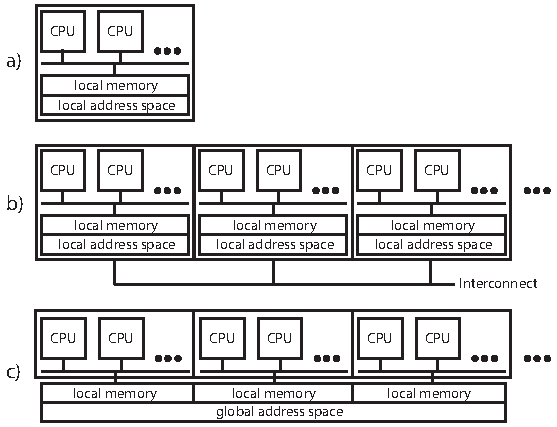
\includegraphics[width=1\textwidth]{Bilder/pgas.pdf}
	\caption{View on a) Shared Memory b) Distributed Memory c) Partitioned Global Address Space}
	\label{pgas_figure}
\end{figure}

Existing PGAS approaches are mainly comprised of dedicated programming languages such as Unified Parallel C (UPC) \cite{upc}, Co-Array Fortran \cite{co_array_fortran} or Chapel \cite{chapel} that allow for compiler optimizations in respect to distributed machines but lack portability and reach. In contrast to this, efforts exist to create libraries for existing programming languages used by many HPC systems.

\section{DASH C++ Template Library}
\label{dash_section}
DASH \cite{dash} is a compiler-free PGAS approach: It consists of a simple C++ library that can be compiled with any C++ compiler and thus can be used out-of-the-box on most HPC systems. The library is part of the Priority Programme ``Software for Exascale Computing'' (SPPEXA)\footnote[1]{http://www.sppexa.de} which supports research on computing systems achieving $10^{18}$ floating point operations per second and above. While PGAS languages require existing programs to be completely rewritten from scratch, DASH allows the applications to be incrementally ported and thus facilitates wider adoption of the PGAS model in the HPC community.

DASH operates on top of the \textit{DASH Runtime} (DART) which is a PGAS memory allocation and communication abstraction written in C. DART enables global memory allocation, pointers to remote memory locations and one-sided communication on top of existing libraries like MPI \cite{mpi3} or GASPI \cite{gaspi}. With DART-MPI \cite{dart_mpi}, a fully functional DART abstraction on top of MPI-3 is used in DASH releases at the time of this writing.

In DASH, processing elements are referred to as \textit{units}. Units can be any processing element such as threads or processes. DASH programs are implemented using the Single Program Multiple Data (SPMD) model: The data is partitioned onto the participating units and each unit executes the same code on its part of the data. Furthermore, units  form \textit{teams} that can be created at runtime. Because HPC hardware topologies become more complex over time (e.g. \cite{dragonfly}), DASH supports hierarchical team creation to allow for a more fine-grained exploitation of data locality compared to the typical local-remote distinction of the PGAS model.

Data is referred to in terms of global pointers and references. A \texttt{GlobPtr<T>} object holds information about the unit and local memory location of the referenced datum. It can be dereferenced to a \texttt{GlobRef<T>} object which behaves like a C++ reference and can be converted to an object of type \texttt{T}. This type conversion triggers a one-sided get operation transferring the data from its remote source to the caller. Similarly, data can be written into the referenced memory location of a \texttt{GlobRef<T>} object.

DASH provides a set of containers for distributed data storage. Aside from the static data structures Array and Matrix, dynamic data structures are available. Since the graph concepts of this work belong into the latter category, details of it are discussed in the following.\\

\subsection{Dynamic memory allocation}
\label{dash_mem_alloc_section}
Dynamic allocation in DASH is encapsulated in the \texttt{GlobHeapMem} concept. \texttt{GlobHeapMem} offers two basic operations to dynamically allocate memory during runtime: \texttt{grow} and \texttt{shrink}. These operations increase or decrease the local size of the memory allocated on the respective unit. Changes in memory space are not reflected in global address space until the operation \texttt{commit} is called which publishes the changes across all units.

A dynamic container in DASH pre-allocates some memory during its initialization. When the  memory is completely used, further additions of elements result in \texttt{GlobHeapMem.grow} operations. A call to the \texttt{barrier} operation of the container results in all newly added elements of the container to be publicly available on all units.\\

Multiple \texttt{grow} operations result in a scattered memory space: Each call to \texttt{grow} creates a new \textit{bucket} - a contiguous memory region in the local freestore. A class implementing the \texttt{GlobHeapMem} concept keeps track of each bucket on each unit so that element indices can be translated to concrete memory locations. \autoref{dash_dynamic_mem_space_figure} illustrates the memory spaces of two units after two grow operations for six elements each have been called. The buckets are allocated at different memory locations. Data access to an element therefore requires the memory location of the bucket and the offset of the element inside the bucket. For this reason, bucket locations and sizes are exchanged between all units during a \texttt{commit} operation and a reference to the object holding the bucket data is needed in every pointer and iterator.

\begin{figure}[ht]
	\centering
  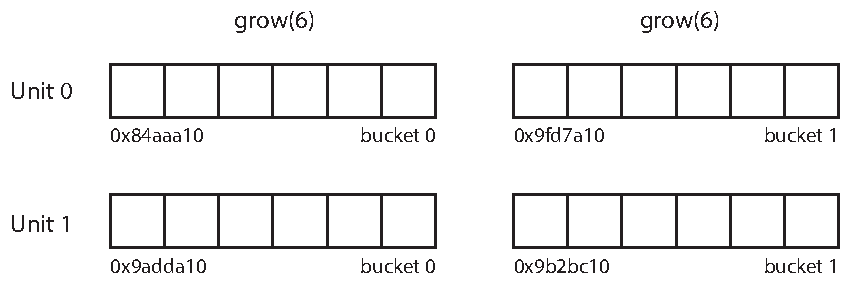
\includegraphics[width=1\textwidth]{Bilder/dash_dynamic_mem_space.pdf}
	\caption{Memory space of two units after two \texttt{GlobHeapMem.grow} operations}
	\label{dash_dynamic_mem_space_figure}
\end{figure}

\chapter{Related Work}
\section{Shared Memory}
\subsection{STINGER}
\subsection{Ligra}
\section{Distributed Memory}
\subsection{Parallel Boost Graph Library}
\subsection{STAPL Parallel Graph Library}

\chapter{Graph Container Concepts}
\label{concept_section}
\section{Fundamentals}
\section{Index Space}
\section{Memory Space}
\label{memspace_section}
\section{Element iteration}
\label{iteration_concept_section}
%http://www.open-std.org/jtc1/sc22/wg21/docs/papers/2011/n3242.pdf ab 718
%hierarchie
\section{Semantics}
%Computational constraints/assumptions

\chapter{Reference Implementation}
\label{impl_section}
This section explains a concrete reference implementation of the concepts in \autoref{concept_section}. The implementation is part of the DASH C++ Template Library and thus written in C++11. It is based on basic C++ concepts illustrated in \autoref{cpp_section}. The reference implementation will be referred to as \texttt{dash::Graph} in this chapter.

\section{Overview}
\texttt{dash::Graph} is part of the dynamic data containers of the DASH Library. As such, it is interacting with existing components of the library. \autoref{impl_overview_figure} depicts the components and their main interactions.\\

\begin{figure}[ht]
	\centering
  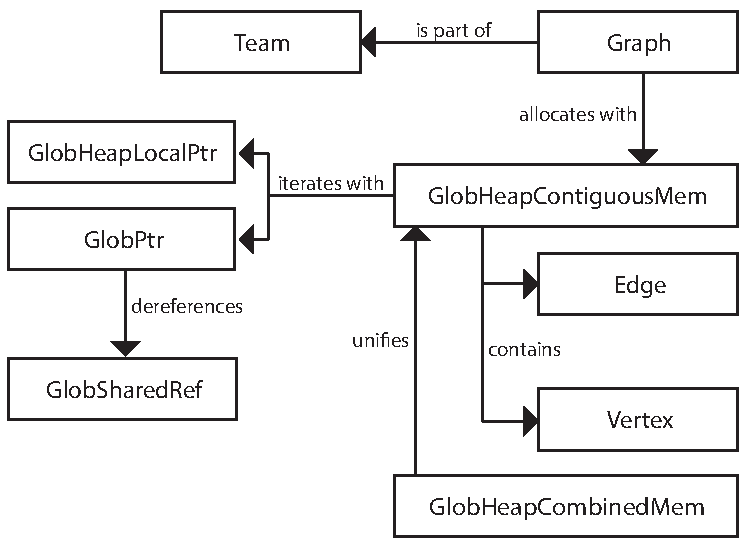
\includegraphics[width=1\textwidth]{Bilder/impl_overview.pdf}
	\caption{dash::Graph component overview}
	\label{impl_overview_figure}
\end{figure}

The \texttt{Graph} gets initialized with a reference to an existing \texttt{Team}. By default, this is \texttt{Team::All()} which includes all units DASH has been initialized with. The \texttt{Graph} creates three instances of \texttt{GlobHeapContiguousMem} for vertices, inbound edges and outbound edges. These instances are used to globally allocate memory for the respective elements. Since the \texttt{Graph} also allows for the iteration of all (inbound and outbound) edges, \texttt{GlobHeapCombinedMem} unifies the memory spaces of the two \texttt{GlobHeapContiguousMem} instances. Both \texttt{GlobHeapContiguousMem} and \texttt{GlobHeapCombinedMem} use a specialized template version of \texttt{GlobPtr} to iterate over the memory space. Each \texttt{GlobPtr} object can then be dereferenced to a \texttt{GlobSharedRef} object which enables direct access to the referenced element. 

\subsection{Pointers and references}
To allow \texttt{GlobPtr} and \texttt{GlobSharedRef} act like real pointers and references respectively, operators like the increment and dereference operators are overloaded. This results in usage analogous to native pointers and references:

\begin{lstlisting}[caption={Operator overloading in GlobPtr and GlobSharedRef}\label{globptr_code}] 
typedef GlobHeapContigousMem<std::vector<int>> g_mem_type;
GlobPtr<int, g_mem_type> ptr(mem, 0);     // position 0 in index space
++ptr;                                    // go to position 1 in index space
auto ref = *ptr;                          // dereference ptr to GlobSharedRef object
int val = ref;                            // convert reference to value
\end{lstlisting}

In this case, \texttt{mem} is an instance of \texttt{GlobHeapContiguousMem} holding at least two globally available elements.

\subsection{Vertices and edges}
Vertices and edges are modeled as individual classes: \texttt{Vertex} and \texttt{Edge}. Each instance of these classes contains objects of the \textit{property} classes defined by the user as template parameters of \texttt{dash::Graph}. The property classes can only contain variables of static size. These variables are filled with default values upon initialization as per \textit{default initialization} of the C++ standard.\\

Additionally, vertices and edges contain their respective index in global index space. The index is not publicly available and can only be read by the \texttt{Graph} class and some of its internal classes. Storing the indices internally is required because of global iteration and remote memory access: After a unit has globally iterated over the elements and dereferenced an element, its index is lost and the user has no way to recover it. The index, however, is needed for various use cases such as iterating over the outbound edges of a certain vertex.

Edges also contain indices of their source and target vertices.\\

\subsection{Graph types}
\label{graph_types_section}
\texttt{dash::Graph} currently supports \textit{directed} and \textit{undirected} graph types. A bidirectional graph type is not implemented but can be integrated later on. As described in \textcolor{red}{LINK CORRECT SECTION}, directed graphs can be instantiated in two different variants depending on the need for inbound edge iteration. This is due to the fact that this iteration is not necessary for most algorithms but requires additional communication that lowers the overall performance of the graph, even if not used at all.

For undirected graphs, edges are replicated to the edge lists of both participating vertices. For directed graphs, the same mechanism is used when inbound edge iteration is needed. Edges in directed graphs without inbound edge iteration are not replicated in any way.

\section{Memory management}
\label{mem_mgmt_section}
\texttt{dash::Graph}'s memory space is handled by \texttt{GlobHeapContiguousMem}. This class follows the concept described in \autoref{memspace_section} but adds an additional feature: Fully contiguous global memory regions. While the memory concept only demands single edge lists to be contiguous, \texttt{GlobHeapContiguousMem} allocates a contiguous memory space for all vertices as well as all edges for better locality exploitation. However, this comes at the expense of additional memory re-allocations in each epoch.

\subsection{Contiguous memory}
\label{contiguous_mem_section}
\autoref{contiguous_mem_figure} illustrates the basic scheme of the contiguous memory allocation. \textit{Region 1} is a publicly available contiguous memory region. The memory location of \textit{Region 1} is known by other units and thus cannot be changed outside of a commit operation. Because of this, \textit{Region 2} is allocated at another memory location that might not be contiguous to \textit{Region 1}. \textit{Region 2} contains elements that have been added in the current epoch - they are available only locally and cannot be seen by other units.

The \texttt{commit} operation starts a new epoch by packing the elements of the two memory regions into another, contiguous memory region and notifying other units about the changed location and size of the region. Traversing the elements in this region is now as simple as incrementing a pointer. Local iteration over the elements however requires a hop between the publicly available region and the local-only region because they are not contiguous. \texttt{GlobHeapLocalPtr} can iterate over an arbitrary number of buckets with contiguous memory (see \autoref{iteration_impl_section}). In this case, always two buckets (the two mentioned memory regions) are used.

\begin{figure}[ht]
	\centering
  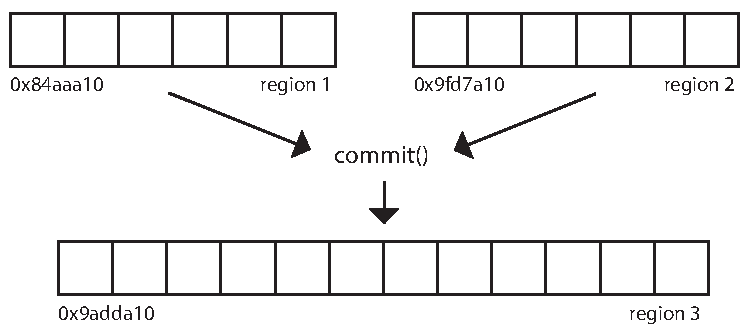
\includegraphics[width=0.9\textwidth]{Bilder/contiguous_mem.pdf}
	\caption{Contiguous memory allocation}
	\label{contiguous_mem_figure}
\end{figure}

\subsection{Edge list memory}
The mechanism in \autoref{contiguous_mem_section} is used for all vertices created at a certain unit. The same mechanism cannot be used for the entirety of all edges created at a single unit, because edge lists have to be contiguous. Appending an element to an edge list would invalidate the offsets of all edges following behind and would also require a re-allocation invalidating the memory location. \autoref{edge_list_insertion_figure} depicts the problem: The new edge inserted at the end of \textit{edge list 1} would be placed at offset 6 in the memory region, incrementing the offsets of all following elements.

\begin{figure}[ht]
	\centering
  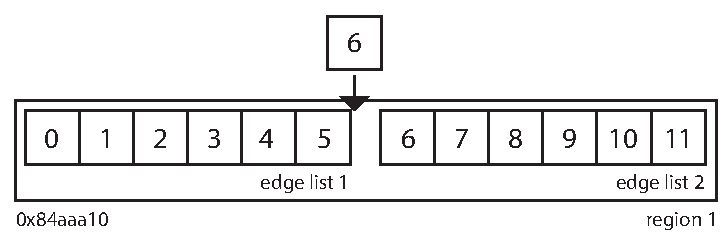
\includegraphics[width=0.9\textwidth]{Bilder/edge_list_insertion.pdf}
	\caption{Element insertion into edge list invalidating offsets}
	\label{edge_list_insertion_figure}
\end{figure}

For this reason, each edge list has to be maintained with individual second regions for element insertions: The mechanism in \autoref{contiguous_mem_section} is used for each edge list individually and the \texttt{commit} operation packs all edge lists into one contiguous memory region.\\

Vertices contain the indices of their respective edge lists and edge list locations and sizes are maintained in \texttt{GlobHeapContiguousMem} so that edge lists of a given vertex can be easily iterated.

\subsection{Element deletion}
Deleting an element in contiguous memory regions requires the its memory location to get invalidated instead of removed to avoid shifting of elements and offset invalidation. If many delete operations occur, the memory space will get scattered. For this reason, it is necessary to take measures that reduce the scattering of the memory to a minimum. \texttt{GlobHeapContiguousMem} uses a \textit{free list}: Deleting an element results in its memory location being added to the free list. If another element is added, a memory location from the back of the free list is used to store the element. Only if the free list is empty, new memory is allocated.

Because invalidated elements are not part of the memory space anymore, iterators have access to the free list so that they can skip the respective elements.

\section{Iteration}
\label{iteration_impl_section}
The four different iteration spaces of the graph concept (see \autoref{iteration_concept_section}) are handled by the same iterator classes. Since the memory space of \texttt{dash::Graph} is epoch-based, iteration space of local iterators can be different to the local part of the iteration space of global iterators.

\subsection{Local iteration}
\label{local_iter_section}
Local iteration in dynamic containers of DASH is handled by \texttt{GlobHeapLocalPtr} that can iterate over multiple non-contiguous memory buckets. \texttt{GlobHeapContiguousMem} holds a list of objects containing bucket meta-data including size and a local native pointer to its beginning memory location. The bucket list is passed to a \texttt{GlobHeapLocalPtr} along with the position the pointer currently holds in the index space of the buckets. The buckets are equal to the allocated memory regions of \texttt{GlobHeapContiguousMem} as described in \autoref{mem_mgmt_section}.

Iteration is done by \texttt{increment}/\texttt{decrement} operations which result in \texttt{GlobHeapLocalPtr} calculating the bucket number the current position belongs to. A \texttt{dereference} operation then accesses the local pointer of the bucket object.

\subsection{Global iteration}
\label{global_iter_section}
For global iteration, a template specialization of \texttt{GlobPtr} for \texttt{GlobHeapContiguousMem} is used. It is similar to the template specialization of \texttt{GlobPtr} for \texttt{GlobHeapMem}, which is used for other dynamic DASH containers like \texttt{dash::List}.

While the bucket meta-data used by \texttt{GlobHeapLocalPtr} contains only information about local buckets, \texttt{GlobPtr} requires information about all buckets on all units. Therefore, \texttt{GlobHeapContiguousMem} distributes bucket information between all units during a \texttt{commit} operation. This information includes bucket sizes as well as DART global pointers to the memory locations of the buckets in global address space. \textcolor{red}{EXPLAIN DART POINTERS?}

With the bucket size information and the DART abstraction of global pointers, \texttt{GlobPtr} can iterate over global memory space the same way as \texttt{GlobHeapLocalPtr} iterates over local memory space. The iteration order is given by the canonical order of units.

\subsection{Edge iteration}
Inbound and outbound edges are handled by separate \texttt{GlobHeapContiguousMem} objects. Iteration of either is therefore handled as described in \autoref{local_iter_section} and \autoref{global_iter_section}. The graph concept however requires iteration over all existing edges. For this reason, \texttt{GlobHeapCombinedMem} is used to unify the iteration spaces of multiple \texttt{GlobHeapContiguousMem} objects.

\begin{figure}[ht]
	\centering
  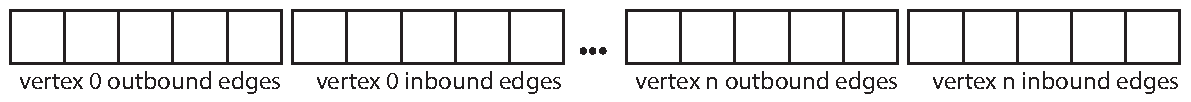
\includegraphics[width=1\textwidth]{Bilder/combined_edges.pdf}
	\caption{Combined edge iteration space}
	\label{combined_edges_figure}
\end{figure}

\autoref{combined_edges_figure} illustrates the order in which the combination of inbound and outbound edges are iterated over.

\section{Data access}
Remote memory data access is strictly handled via \texttt{GlobSharedRef} objects. These objects issue DART \texttt{get}/\texttt{put} operations to access data on remote machines. If referenced data resides locally, \texttt{GlobSharedRef} directly accesses it in the memory.

Because edges are replicated for some graph types (see \autoref{graph_types_section}), writing data to an element with a \texttt{GlobSharedRef} object would introduce consistency problems because it is restricted to referencing single memory locations. \texttt{GlobSymValue} \textcolor{red}{ADAPT NAME ONCE DEFINED} is set up with two DART global pointers to account for this problem. An assignment to a \texttt{GlobSymValue} object results in two memory locations being updated.


\chapter{Case studies}
\section{Static structure}
\subsection{Graph traversal}
\subsection{Shortest path evaluation}
\section{Dynamic Structure}
\subsection{Graph partitioning}
\subsection{De Bruijn Graph construction}

\chapter{Evaluation}
\section{Micro-benchmarks}

\chapter{Conclusion}
\section{Summary}
\section{Assessment}
\section{Outlook}

% ---------------------------------------------------------------
\backmatter % ab hier keine Nummerierung mehr
    \listoffigures
    \bibliographystyle{alphadin}
    \bibliography{./Bib/effe17}

\end{document}
